\section{Tasks}

During our user tests, we need to ask participants to provide a subjective assessment of their experience using our \textbf{Assistant}. There are several widely used questionnaires giving us different prons-and-cons. However, in most cases, a \hyperlink{https://www.nngroup.com/articles/keep-online-surveys-short/}{single question instrument}~\cite{sauro201210} is the right method for a quantitative usability testing. By taking less time and effort to answer, participants are pursuing to this phase after task while it is minimally disruptive.

\clearpage

%%%%%%%%%%%%%%%%%%%%%%%%%%%%%%%%%%%%%%%%%%%%%%%%%%%

\hfill

\begin{wrapfigure}{r}{0.50\textwidth}
\centering
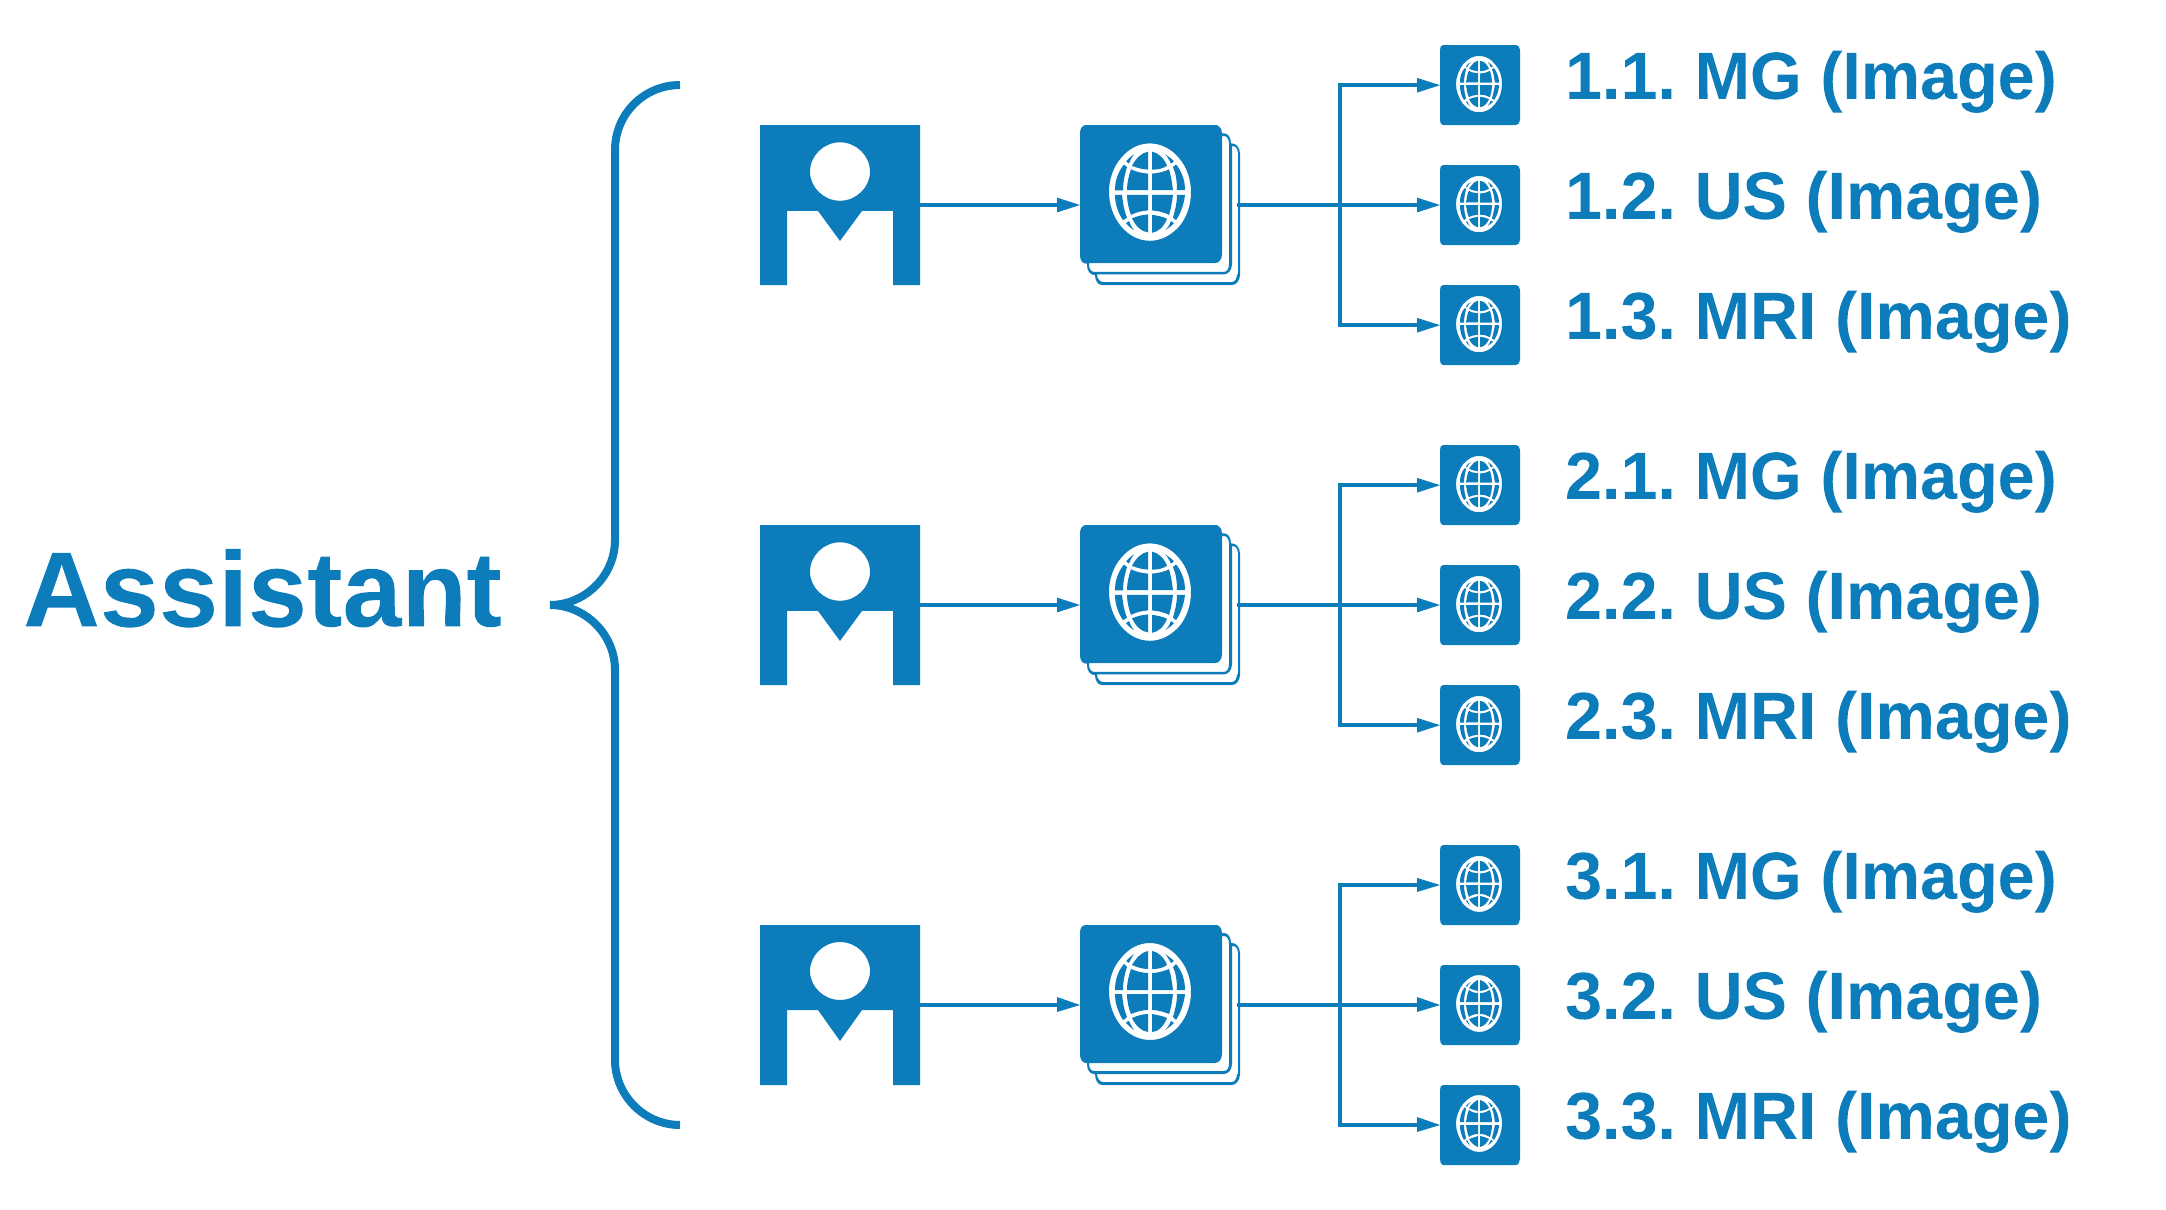
\includegraphics[width=0.50\textwidth]{img001}
\caption{Diagram representing the use of the \textbf{Assistant} by clinicians.}
\label{fig:svmm}
\end{wrapfigure}

\hfill

%%%%%%%%%%%%%%%%%%%%%%%%%%%%%%%%%%%%%%%%%%%%%%%%%%%

We will try to understand if, with the \textit{AI-Assisted} techniques, the clinicians will encounters the most accurate severity (\hyperlink{https://en.wikipedia.org/wiki/BI-RADS}{BIRADS}) of the breast lesions~\cite{american1998breast} and patient's prognostic. For this purpose, we have three patients (Figure \ref{fig:svmm}); each patient has three images in the respective modalities: (i) MG; (ii) US; and (iii) MRI. The clinicians will proceed to the activity of diagnosing the three patients within the support of our \textbf{Assistant} by the observation of ALL images.

\hfill

In our \textbf{User Testing Guide} a set of tasks is necessary and carefully crafted. Our test studies involve asking participants to perform a set of tasks. By looking at what our user need to do with our system, our tasks are realistic as possible. We are not describing the exact steps participants need to take. We achieve that by avoiding the precise language used as labels in our system. The tasks are emotionally neutrals. And we did several \hyperlink{https://www.nngroup.com/articles/pilot-testing/}{pilot tests} to prevent misleading situations saving us from wasting resources by accidentally use a lousy task or from getting bad data. The tasks are as follows.

\hfill

%%%%%%%%%%%%%%%%%%%%%%%%%%%%%%%%%%%%%%%%%%%%%%%%%%%

List of stand alone tasks:

%%%%%%%%%%%%%%%%%%%%%%%%%%%%%%%%%%%%%%%%%%%%%%%%%%%

\hfill

\begin{itemize}
\item[] \textbf{Task 1.1:} Classify \textit{Patient 1} on the \textbf{Assistant};
\item[] \textbf{Task 1.2:} Classify \textit{Patient 2} on the \textbf{Assistant};
\item[] \textbf{Task 1.3:} Classify \textit{Patient 3} on the \textbf{Assistant};
\end{itemize}

\hfill

\begin{itemize}
\item[] \textbf{Task 2.1:} Freely explore \textit{Patient 1} on the \textbf{Assistant};
\item[] \textbf{Task 2.2:} Freely explore \textit{Patient 2} on the \textbf{Assistant};
\item[] \textbf{Task 2.3:} Freely explore \textit{Patient 3} on the \textbf{Assistant};
\end{itemize}

\hfill

%%%%%%%%%%%%%%%%%%%%%%%%%%%%%%%%%%%%%%%%%%%%%%%%%%%
























%%%%%%%%%%%%%%%%%%%%%%%%%%%%%%%%%%%%%%%%%%%%%%%%%%%
%                                                 %
%                     SECTION                     %
%                                                 %
%%%%%%%%%%%%%%%%%%%%%%%%%%%%%%%%%%%%%%%%%%%%%%%%%%%

\subsection{Case Studies}

The functionality of the prototype will be best demonstrated by a series of case studies. By describing the expected workflow and capabilities of the research study at the \textbf{RR} specific environment and changes of the workflow by using our system prototype. The study implies the evaluation of medical imaging \textit{AI-Assisted} features on several breast lesions. The primary goal of this case studies analysis is to generate a receiver operating characteristic to evaluate the performance and validation of our \textbf{Assistant}. Let us consider a list of hypothetical use cases for the research investigation that evaluates the interaction and usability performance of the \textbf{Assistant}. Therefore, the following list will show the preliminary case studies.

\hfill

List of case studies to analyse our solution prototype:

\hfill

\begin{itemize}
\item Multi-Modality \textit{AI-Assisted} of a Breast Cancer Diagnosis;
\item Priority \& Minimal Information Visualisation;
\item Performance \& Response Measurement Values Acquisition;
\item Radiologist Validation;
\end{itemize}

\hfill

%%%%%%%%%%%%%%%%%%%%%%%%%%%%%%%%%%%%%%%%%%%%%%%%%%%

We expect to demonstrate several uses through a series of case studies, including implementation of our research prototype using an \textit{AI-Assisted} technique and features for several view studies and other imaging research, as well as creation of a novel \textbf{Assistant} for the purpose. By creating a set of questions, we will try to achieve and feed this case studies. It is automatically associated with all cases. The radiologist may interact with our \textbf{Assistant} while manipulating the medical imaging and report to us difficulties and improvements. The number of questions is not restricted to the present document, since the interview will be open and suggestive~\cite{joyce2017healthcare}. There is no limit to the number of questions that can be asked per case but it should fit the amount of expected time per each.

The data will be collect from the study video and observations into a \hyperlink{https://docs.google.com/spreadsheets/d/1CoPLONnINdBWryGs7SBRuPZA-DnQ0t_yzx3u8ym0UoI/edit?usp=sharing}{spreadsheet} for further analysis. We will \hyperlink{https://github.com/mida-project/research-reports}{report} the results of this tests and conclusions. This guide and respective use cases will be iteratively improved.

























%%%%%%%%%%%%%%%%%%%%%%%%%%%%%%%%%%%%%%%%%%%%%%%%%%%
%                                                 %
%                     SECTION                     %
%                                                 %
%%%%%%%%%%%%%%%%%%%%%%%%%%%%%%%%%%%%%%%%%%%%%%%%%%%

\subsection{Devices}

Traditional interaction remains the most common way to interact with user interfaces in a clinical environment. Unfortunately, most of this interaction is made by low profile equipment that makes users produce more errors and take more time interacting with those User Interfaces (UI).

For this \textit{User Testing Guide}, we will use the \hyperlink{https://gaming.tobii.com/product/tobii-eye-tracker-4c/}{Tobii Eye Tracker 4C} (\hyperlink{https://www.tobii.com/}{Tobii}, Sweden). This device, is a remote eye tracking device that provides an estimate of the point-gaze and 3D eye position for each eye at 90Hz. We will attach the eye tracker under the display area with a magnetic mounting bracket, following the product's instructions. A 9-point calibration~\cite{chatelain2018evaluation} will be performed for each user. Our protocol was implemented in \hyperlink{https://www.python.org/}{Python} (\textit{versions} $>=$ \hyperlink{https://docs.python.org/2/}{v2.7}) and \hyperlink{http://www.processing.org/}{Processing} (\textit{versions} $>=$ \hyperlink{https://github.com/processing/processing/releases/tag/processing-0269-3.5.3}{v3.5.3}). The setup repository was the \hyperlink{https://github.com/mida-project/eye-tracker-setup}{eye-tracker-setup}, while the repository to measure and calculate the setup gazing information was the \hyperlink{https://github.com/mida-project/eye-tracker-naive}{eye-tracker-naive} repository.

\clearpage

On Figure \ref{fig:patient_list}, the user can select the list of patients. The list has a table with several patient information. The first column is the \textit{Patient ID}; we used it as an identifier of the patient. In that way, we can have anonymized information with no reference to the patient name. The second column is the \textit{Study Date}, the third column is the \textit{Modality} of the used \textbf{DICOM} image, the fourth column is the \textit{Study Description} of the used study and the last column is the number of \textit{Images}.

%%%%%%%%%%%%%%%%%%%%%%%%%%%%%%%%%%%%%%%%%%%%%%%%%%%

\hfill

\begin{figure}[h]
\centering
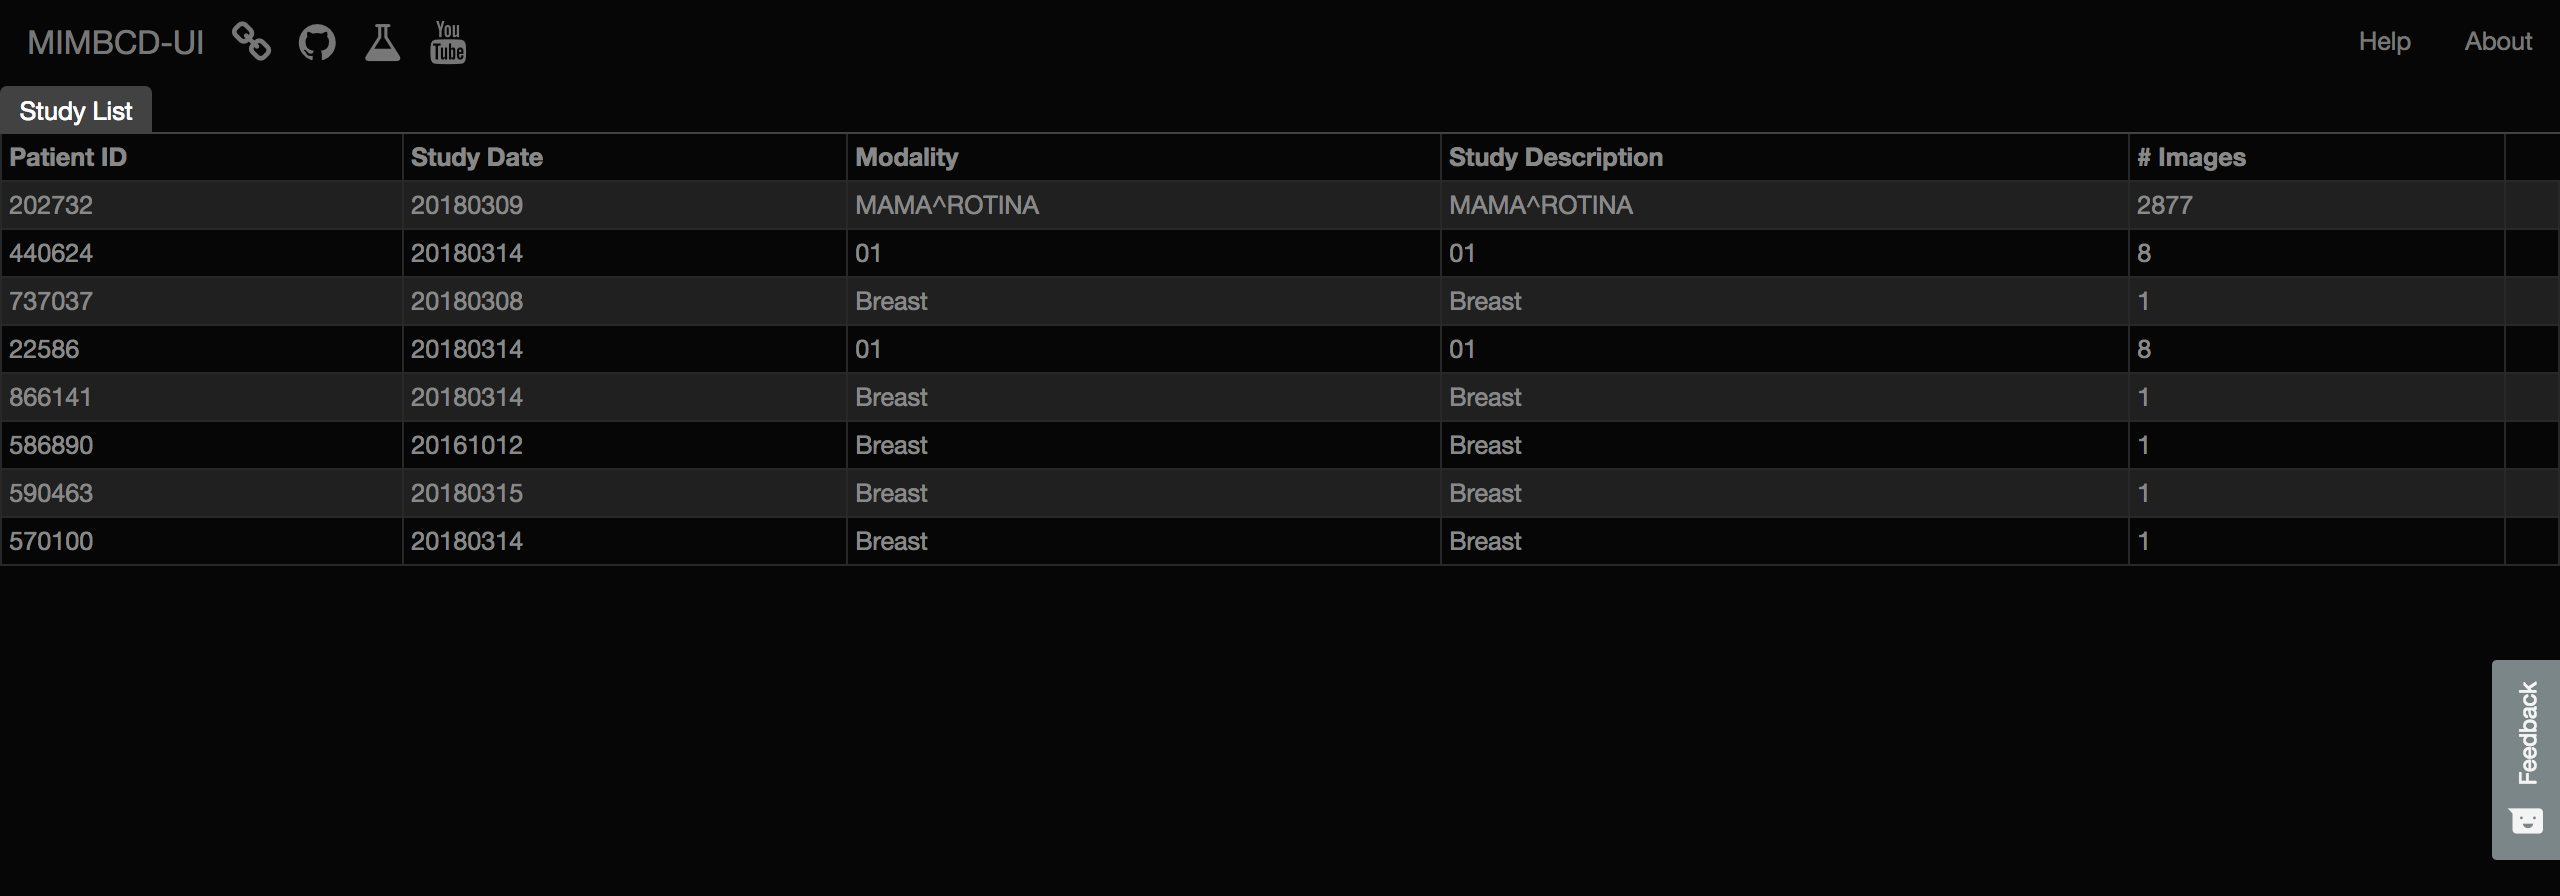
\includegraphics[width=\textwidth]{patient_list}
\caption{List of Patients.}
\label{fig:patient_list}
\end{figure}

\hfill

%%%%%%%%%%%%%%%%%%%%%%%%%%%%%%%%%%%%%%%%%%%%%%%%%%%

As we can see in Figure \ref{fig:image_viewer}, it shows the first task in our User Interface (UI), where the patient's breasts are on a small left column. The options are in a short row near of the viewport and described below. We also have the tabs where the user can change the patient. The centre viewport shows the \textbf{DICOM} image, and it can be configured to display a number up to four \textbf{DICOM} images at the same time. The viewport has some text information on it (yellow) with the details of the metadata. Nevertheless, the \textit{Assistant} suggestions are shown on the top-right corner of the system. Our \textit{Assistant} system allows a doctor-bot to provide a second opinion about the image severity of each patient. In other words, the \textit{Assistant} is an Artificial Intelligence (AI) engine to interact with clinicians. It has an interface, wherein a representation of a doctor, presenting with a text box. The \textit{Assistant} system is, therefore, made to diagnose and provide a second opinion for lesion severities of the breast cancer diseases.

\clearpage

%%%%%%%%%%%%%%%%%%%%%%%%%%%%%%%%%%%%%%%%%%%%%%%%%%%

\hfill

\begin{figure}[h]
\centering
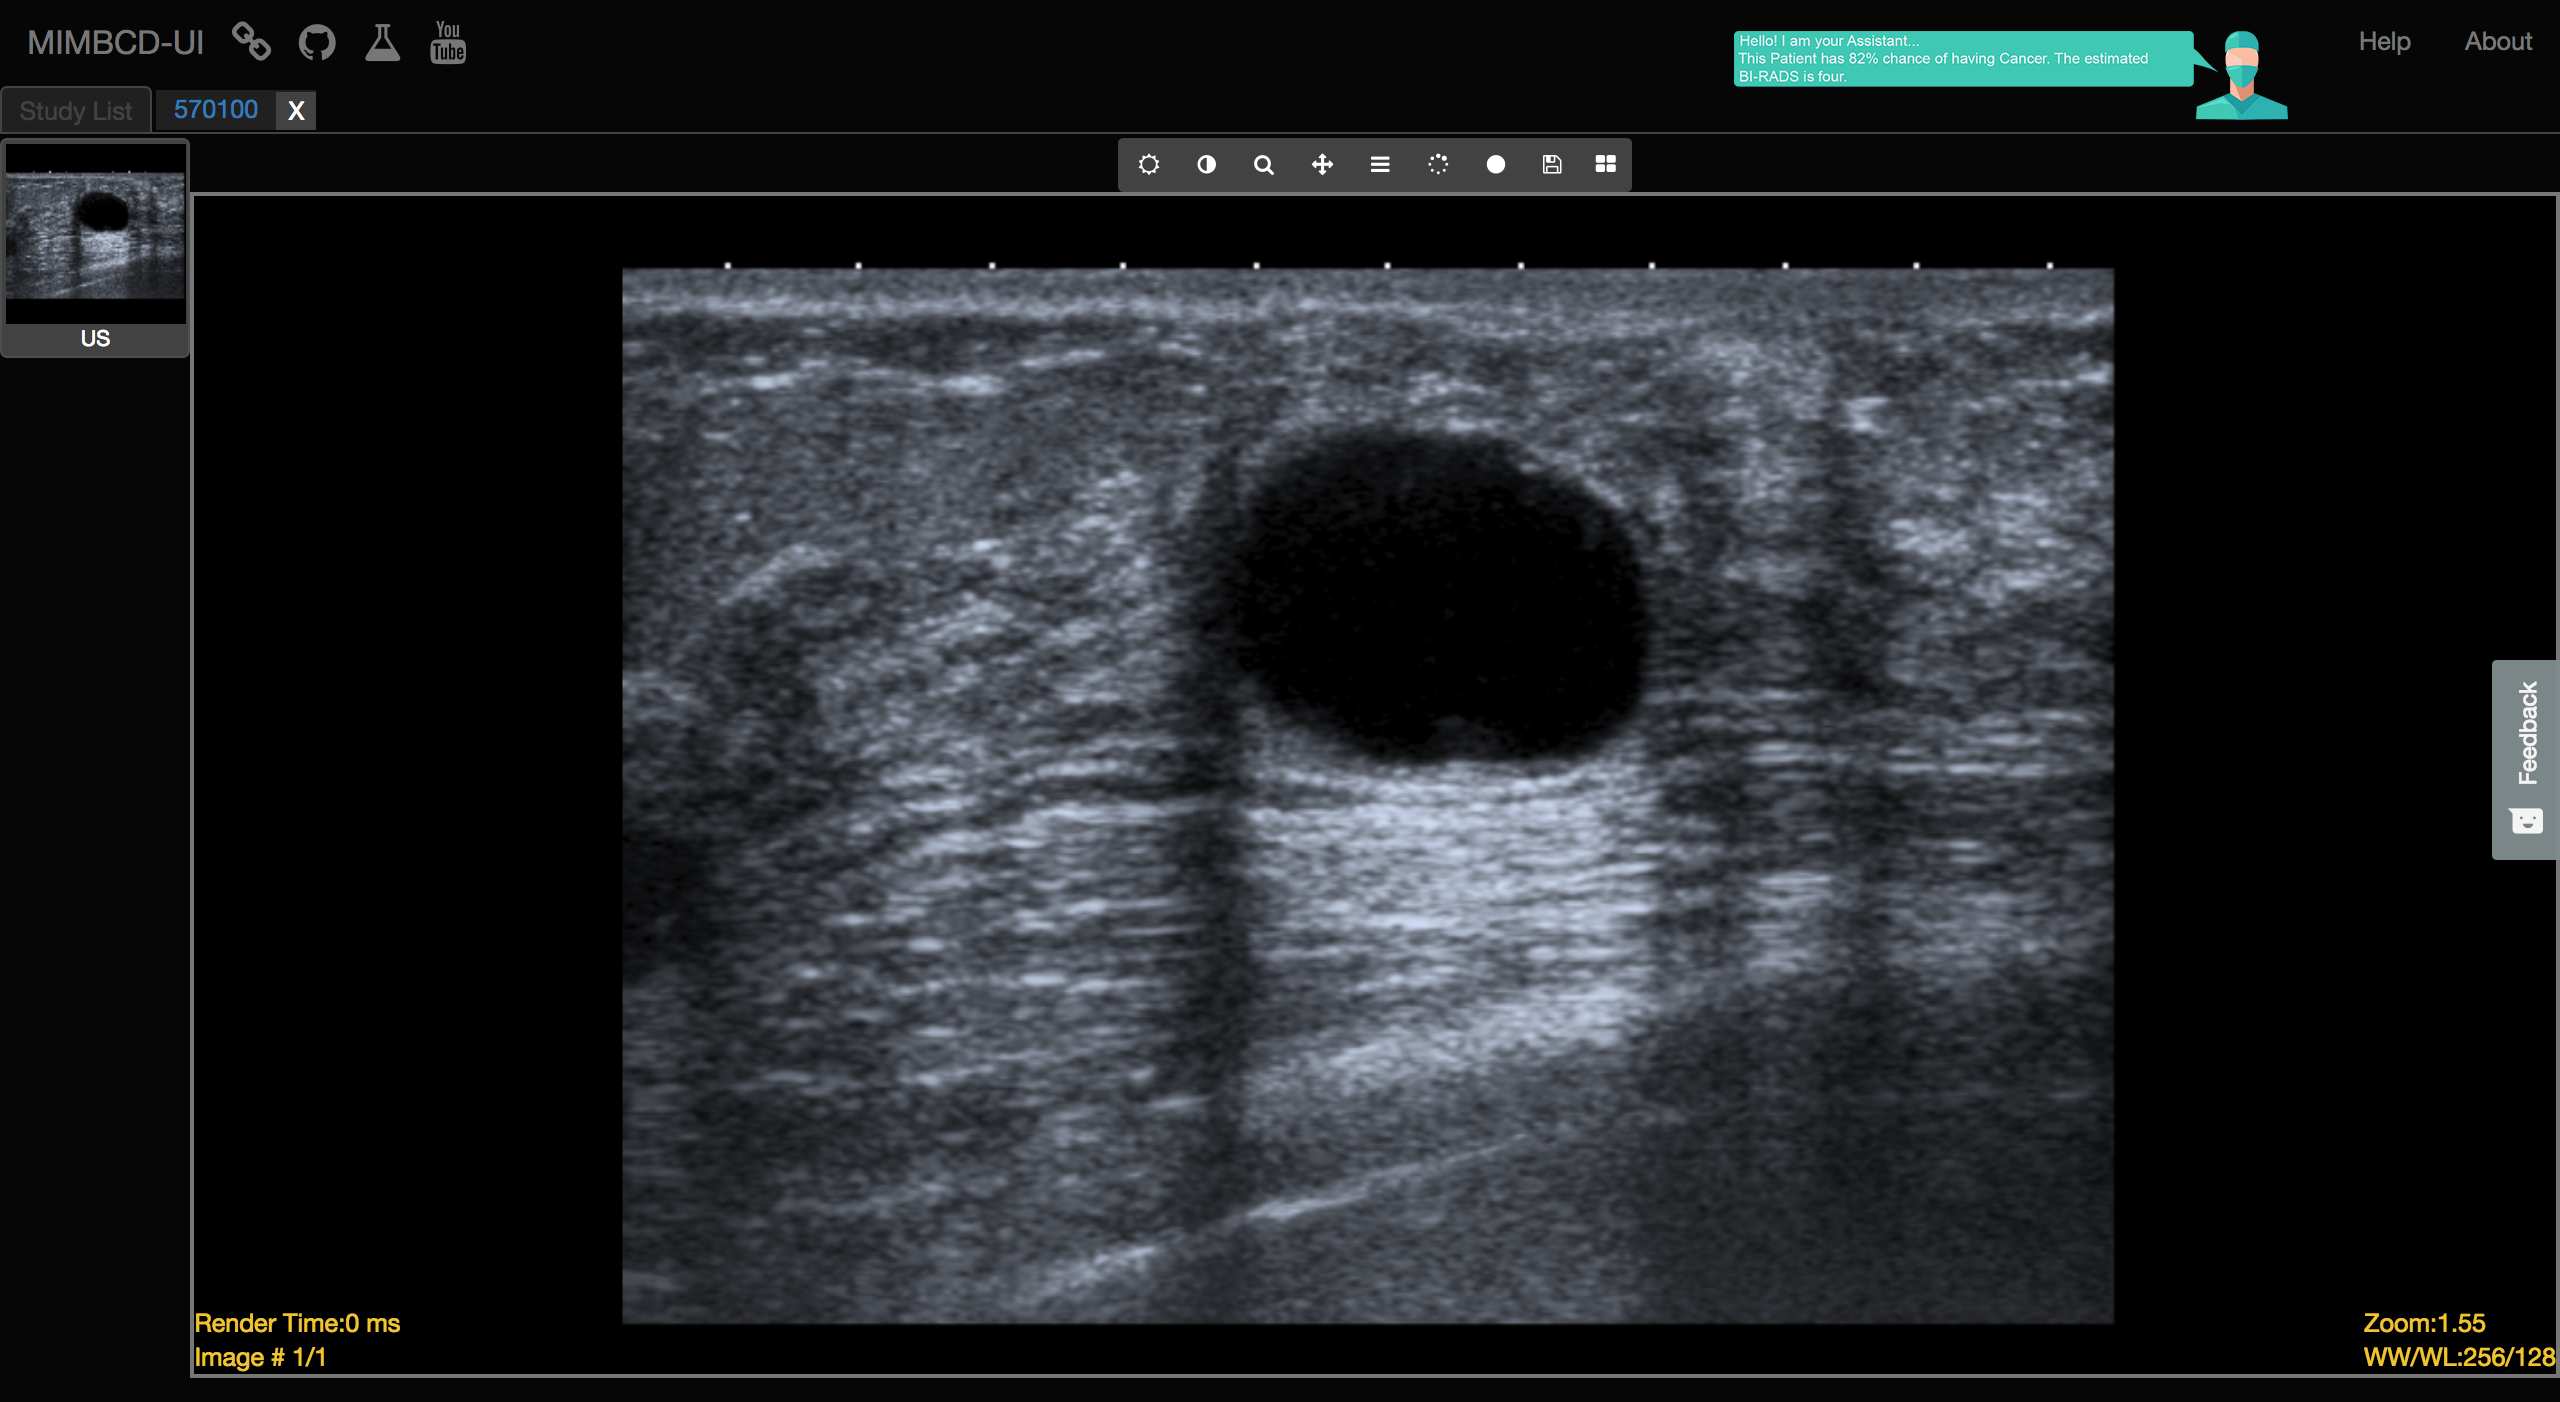
\includegraphics[width=\textwidth]{image_viewer}
\caption{Viewer of the \textbf{DICOM} images.}
\label{fig:image_viewer}
\end{figure}

\hfill

%%%%%%%%%%%%%%%%%%%%%%%%%%%%%%%%%%%%%%%%%%%%%%%%%%%

Manual annotation~\citation{cao2015collaborative} is adopted by us thanks to Freehand ROI and Probe annotation features, both from \hyperlink{https://cornerstonejs.org/}{CornerstoneJS}. According to the \hyperlink{https://cornerstonejs.org/}{CornerstoneJS} Library, the user can create an annotation by setting up consecutive landmarks around a Region of Interest (ROI). The markers finish a lesion annotation when it interconnects the last bullet point. Additional features, available in our User Interface (UI), includes on-demand increment of the number of landmarks, and throw transformations of the shape of an annotation. For the \textit{Assistant} (\textbf{Sce2.}), we provide the recommendations of our \textit{bot-like} system. This \textit{bot-like} will give clinicians informatiuon regarding the patient's achieved severity of the breast (\hyperlink{https://en.wikipedia.org/wiki/BI-RADS}{BIRADS}), and the respective interpretation by text. The interpretation can be simple analysis of the patient's co-variables. A further analysis, when we show the heatmap answer (\hyperlink{https://github.com/mida-project/prototype-heatmap}{prototype-heatmap} repository), will provide explainability to clinicians concerning the lesion severities across each image.

\clearpage

%%%%%%%%%%%%%%%%%%%%%%%%%%%%%%%%%%%%%%%%%%%%%%%%%%%
%                                                 %
%                     SECTION                     %
%                                                 %
%%%%%%%%%%%%%%%%%%%%%%%%%%%%%%%%%%%%%%%%%%%%%%%%%%%

\subsection{User Interactions}

The systems have several buttons (Figure \ref{fig:toolbar}) that allows the user to interact or access to a set of user interface features. Each item of the following list represents each metaphoric icon of Figure \ref{fig:toolbar}.

%%%%%%%%%%%%%%%%%%%%%%%%%%%%%%%%%%%%%%%%%%%%%%%%%%%

\hfill

\begin{figure}[h]
\centering

\includegraphics[width=\textwidth]{toolbar}
\caption{Toolbar of the System available features.}
\label{fig:toolbar}
\end{figure}

\hfill

%%%%%%%%%%%%%%%%%%%%%%%%%%%%%%%%%%%%%%%%%%%%%%%%%%%

\hfill

The buttons are (from left to right of Figure \ref{fig:toolbar}) as follows:

\hfill

\begin{itemize}
\item WW/WC
\item Invert
\item Zoom
\item Pan
\item Stack Scroll
\item Freehand
\item Probe
\item Save
\item Window Controller
\end{itemize}

\hfill

\clearpage























%%%%%%%%%%%%%%%%%%%%%%%%%%%%%%%%%%%%%%%%%%%%%%%%%%%

%%%%%%%%%%%%%%%%%%%%%%%%%%%%%%%%%%%%%%%%%%%%%%%%%%%
%                                                 %
%                     SECTION                     %
%                                                 %
%%%%%%%%%%%%%%%%%%%%%%%%%%%%%%%%%%%%%%%%%%%%%%%%%%%

\subsection{Post-Task Questionnaire}

Our metrics will refer the \textit{AI-Assisted} involvement against specific goals necessary to satisfy several requirements of our \textbf{Assistant}. For our \textbf{Post-Task Questionnaire} we will use \textit{Quantitative Analysis} (QtA) and \textit{Qualitative Analysis} (QlA) in response to our questions (Section \ref{sec:sec003}) to measure the acceptability of our \textbf{Assistant} each time a \textit{scenario} is completed (Section \ref{sec:sec003}). From a set of tasks (Section \ref{sec:sec006}) we aim to cover our main scenario, an \textit{AI-Assisted} that we call \textbf{Assistant}. Therefore, both QtA and QlA will allow the facilitator to quickly and easily assess the requirements of the given scenario. Our QtA and QlA requirements will have several attributes~\cite{joyce2017healthcare} that make it a good choice for our clinical participants. Those attributes are as follows.

\hfill

%%%%%%%%%%%%%%%%%%%%%%%%%%%%%%%%%%%%%%%%%%%%%%%%%%%

List of the scale attributes:

%%%%%%%%%%%%%%%%%%%%%%%%%%%%%%%%%%%%%%%%%%%%%%%%%%%

\hfill

\begin{itemize}
  \item The requirements are technology agnostic, making it flexible enough;
  \item The requirements are relatively quick and easy to answer;
  \item The requirements provide a single score on a scale that is easily understood;
  \item The requirements are nonproprietary, making it a cost effective tool;
\end{itemize}

\hfill

%%%%%%%%%%%%%%%%%%%%%%%%%%%%%%%%%%%%%%%%%%%%%%%%%%%

\clearpage

The facilitator will explain that the amount of time taken to complete the \textit{tasks} will be measured and that exploratory behaviour outside the \textit{task} flow should not occur until after task completion. At the beginning of each task, the participant will listen the \textit{task} description from the facilitator and begin the task. \textit{Time-on-Task} (ToT) measurements begins when the participant starts the \textit{task}, measured until the end of each \textit{task}.

%%%%%%%%%%%%%%%%%%%%%%%%%%%%%%%%%%%%%%%%%%%%%%%%%%%

%%%%%%%%%%%%%%%%%%%%%%%%%%%%%%%%%%%%%%%%%%%%%%%%%%%
%                                                 %
%                     SECTION                     %
%                                                 %
%%%%%%%%%%%%%%%%%%%%%%%%%%%%%%%%%%%%%%%%%%%%%%%%%%%

\subsection{Training Session}

The participant will receive and overview the test procedure. However, the user will not receive information how to annotate and interact in all degrees of freedom. With the aim of disabling users to get their work done before the test tasks. It will take advantage of a "surprise" acknowledgement.

%%%%%%%%%%%%%%%%%%%%%%%%%%%%%%%%%%%%%%%%%%%%%%%%%%%
%                                                 %
%                     SECTION                     %
%                                                 %
%%%%%%%%%%%%%%%%%%%%%%%%%%%%%%%%%%%%%%%%%%%%%%%%%%%

\subsection{Execution of Tasks}

The \textit{tasks} were derived from test scenarios developed from \textbf{Case Studies}. Due to the range and extent of functionality provided by our \textbf{Assistant}, and the short time from which each participant will be available, the \textit{tasks} are the most common and relatively complex of available functions. The \textit{tasks} are the identical for all participants of a given user role in the study.

The \textit{tasks} will be performed by several classes of radiology experience. Professionals from Radiology Seniors, Middles, Juniors and Interns will be performing these \textit{tasks}. On the \textbf{RR} the Radiologist is characterised~\cite{ehrlich2016patient, miglioretti2007radiologist} as a physician who examines and interpret Medical Imaging (MI) \cite{kobashi2017evaluation}, such as X-Rays, CT Scans or MRIs.

%%%%%%%%%%%%%%%%%%%%%%%%%%%%%%%%%%%%%%%%%%%%%%%%%%%

%%%%%%%%%%%%%%%%%%%%%%%%%%%%%%%%%%%%%%%%%%%%%%%%%%%
%                                                 %
%                     SECTION                     %
%                                                 %
%%%%%%%%%%%%%%%%%%%%%%%%%%%%%%%%%%%%%%%%%%%%%%%%%%%

\subsection{Post-Activity Questionnaire}

After completing all \textit{tasks} and scenarios, participants will be asked to complete a questionnaire to classify the \textbf{Assistant} according to various parameters regarding the several features. To measure this, we will use an open session \textit{observation} and \textit{interview}~\cite{carayon2015systematic}. We will use this techniques to identify participants' requirements during the various stages of the workflow.

%%%%%%%%%%%%%%%%%%%%%%%%%%%%%%%%%%%%%%%%%%%%%%%%%%%












\section{Measurements}
\label{sec:sec007}

Our measurements refers to user performance measured against specific performance goals necessary to satisfy requirements. \textit{Task} completion success rates, adherence to dialog scripts, error rates and subjective evaluations will be used. \textit{Time-to-Completion} (TtC) of \textit{tasks} will also be collected. The measures are as follows.

\hfill

%%%%%%%%%%%%%%%%%%%%%%%%%%%%%%%%%%%%%%%%%%%%%%%%%%%

The tests are intended to achieve the following measures:

%%%%%%%%%%%%%%%%%%%%%%%%%%%%%%%%%%%%%%%%%%%%%%%%%%%

\hfill

\begin{itemize}
\item BIRADS Classification;
\item Pathology Classification;
\item Time measurement;
\item Number of clicks;
\item Number of errors;
\item Efficiency;
\item Difficulty;
\item Experience;
\end{itemize}

\hfill

%%%%%%%%%%%%%%%%%%%%%%%%%%%%%%%%%%%%%%%%%%%%%%%%%%%

To prioritise recommendations, a method for problem difficulty and degree severity classification, as well as, pathology importance, will be used in the analysis of the collected data during evaluation process. The approach treats problem severity has a combination of several factors. Those factors are measuring the impact of the problem and the frequency of users experiencing issues during the evaluation. Nevertheless, the opinion will also be of chief importance and we will also register the received ones.

\hfill

%%%%%%%%%%%%%%%%%%%%%%%%%%%%%%%%%%%%%%%%%%%%%%%%%%%

Through the questionnaire after the test session, we intend to obtain the answers to the following questions for each \textit{task}:

%%%%%%%%%%%%%%%%%%%%%%%%%%%%%%%%%%%%%%%%%%%%%%%%%%%

\hfill

\begin{itemize}
\item Acceptability of the \textbf{Assistant} lesion classification;
\item Acceptability of the \textbf{Assistant} interaction;
\item Acceptability of the \textbf{Assistant} translation;
\item Acceptability of the \textbf{Assistant} available features;
\item \textbf{Assistant} degrees of classification;
\item \textbf{Assistant} degrees of interaction;
\item \textbf{Assistant} degrees of information visualisation;
\end{itemize}

\hfill

%%%%%%%%%%%%%%%%%%%%%%%%%%%%%%%%%%%%%%%%%%%%%%%%%%%